\documentclass{article}
\usepackage[utf8]{inputenc}
\usepackage[english]{babel}
\usepackage[]{amsthm} 
\usepackage[]{amssymb} 
\usepackage{amsmath}
\usepackage{graphicx}
\usepackage{hyperref}
\usepackage{mathtools}
\usepackage[thinc]{esdiff}
\usepackage[dvipsnames]{xcolor}
\usepackage{float}
\usepackage{listings}
\usepackage{tcolorbox}
\usepackage{listings}
\usepackage{xcolor}
\usepackage{xparse}

\NewDocumentCommand{\codeword}{v}{%
\texttt{\textcolor{blue}{#1}}%
}

\lstset{language=Python,keywordstyle={\bfseries \color{blue}}}

\graphicspath{ {./HW5_img/} }
\setcounter{MaxMatrixCols}{16}

\title{ADSP: HW5}
\author{Lo Chun, Chou \\ R13922136}
\date\today


\begin{document}
\setlength{\parindent}{0pt}
\maketitle 

\tcbset{
    greenbox/.style={
        colback=SpringGreen!20,
        colframe=SpringGreen!80,
        coltitle=black,
        sharp corners
    },
    bluebox/.style={
        colback=SkyBlue!20,
        colframe=SkyBlue!80,
        coltitle=black,
        sharp corners
    },
    yellowbox/.style={
        colback=yellow!10,
        colframe=yellow!80,
        coltitle=black,
        sharp corners
    }
}


\section*{(1)}

An example result of the code is shown as the following image:

\begin{figure}[H]
    \centering
    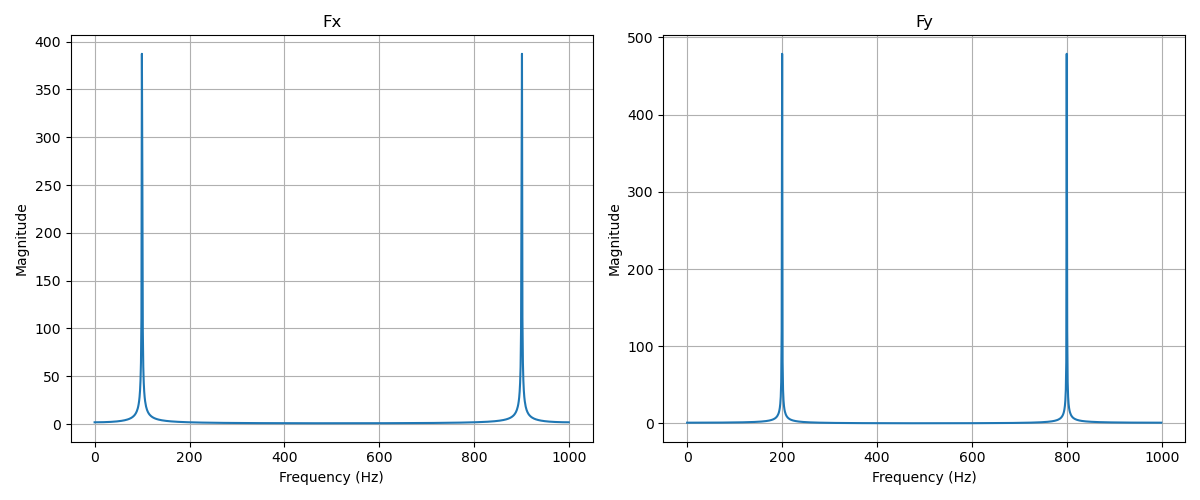
\includegraphics[width=\textwidth]{problem_1/prob1_result.png}
\end{figure}

For the code, please refer to the attached python file \codeword{problem_1.py} on NTUCOOL.

\section*{(2)}

The two main advantages of the sectioned convolution 
compared with the original non-sectioned convolutions are:

\begin{itemize}
    \item We can reduce computation by sectioning, since the complexity of sectioned convolution is linear with $N$ ($\mathbb{\theta}(N)$),
    however, for non-sectioned convolution, the complexity is $\mathbb{\theta}(N \log N)$
    \item Since the restriction $P \geq M + N - 1$ needs to be satisfied, 
    when the number of $N$ changes, the number of $P$ should also change.
    \bigskip

    Even though this could be easily implemented by software, 
    it is not realistic for hardware implementation,
    because implementing multiple fourier transforms on a chip with different $N$s, 
    in order to deal with inputs of different length is too costly.
    \bigskip

    However, if we split the input signal into multiple sections,
    with each section of length $L$, 
    for the number of points of the fourier transform ($P$) to satisfy the inequality $P \geq M + L - 1$, 
    since $L$ is fixed, $P$ would not be affected by the length of the input signal $N$.
\end{itemize}

\section*{(3)}

To compute the convolution operation of $y[n] =  x[n] * h[n]$, where:

\begin{align*}
    h[n] = [0.09 \ 0.36 \ 0.55 \ 0.55 \ 0.36 \ 0.09] \quad -2 \leq n \leq 3 
\end{align*}

by an efficient way that the number of multiplciations is minimized, 
first observe that $h[n]$ is symmetric, 
since it fits the two conditions in lecture note "ADSP\_Write6.pdf", p.439: 

\begin{itemize}
    \item $M$ is small
    \item The filter has some symmetric relation
\end{itemize}

This is the case that we can use "direct computing" to compute the convolution operation:

\begin{align*}
    y[n] 
    &= 
    \textcolor{Green}{0.09 x[n - 3]} + 
    \textcolor{blue}{0.36 x[n - 2]} + 
    \textcolor{orange}{0.55 x[n - 1]} + 
    \textcolor{orange}{0.55 x[n]} + 
    \textcolor{blue}{0.36 x[n + 1]} + 
    \textcolor{Green}{0.09 x[n + 2]} \\
    &= 
    \textcolor{Green}{0.09 (x[n - 3] + x[n + 2])} + 
    \textcolor{blue}{0.36 (x[n - 2] + x[n + 1])} + 
    \textcolor{orange}{0.55 (x[n - 1] + x[n])} \\
\end{align*}


\section*{(4)}

Given that the $\mathrm{length}(x[n]) = 1500$, 
we can find the optimal approach by the cases in lecture note "ADSP\_Write6.pdf", p.437, 441.
And the following are the formulas showing the amount of multiplications for each case:
\bigskip
\begin{itemize}
\item For direct computing, we have:

\begin{align*}
    3N \times M, \qquad \text{where } N = \mathrm{length}(x[n]), \ M = \mathrm{length}(h[n])
\end{align*}

\item If we use non-sectioned convolution, which is $y[n] = \mathrm{IFFT}_P( \mathrm{FFT}_P\{x[n]\} \times \mathrm{FFT}_P\{h[n]\} )$

\begin{align*}
    2 \times \mathrm{MUL}_{P} + 3 P, \qquad \text{where } P \geq N + M - 1
\end{align*}

\item If we use sectioned convolution, we have;

\begin{align*}
    S \times (2 \times \mathrm{MUL}_{P} + 3 P), \qquad \text{where } S = \left\lceil \frac{N}{L} \right\rceil
\end{align*}

\end{itemize}

Since the values are large and hard to calculate by hand, 
I wrote a python code to calculate the results of the three approaches.
\bigskip

Instead of showing the code here, 
I attached the code to NTUCOOL since it's too long.

Also, In the following subproblems, I will show the output for executing the code, 
which shows detailed process for finding the optimal approach.
If the code needs to be executed and checked, 
execute \codeword{python 4.py}, 
and modify the input parameters \codeword{N} and \codeword{M} to get the results:

\begin{figure}[H]
    \centering
    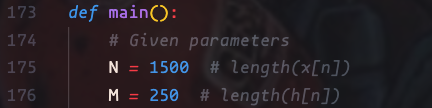
\includegraphics[width=0.6\textwidth]{problem_4/code_input_setting.png}
\end{figure}

Another thing is that, since the output is also quite lengthy, 
the answer is written after the output.

\subsection*{(a)}

If $\mathrm{length}(y[n]) = 250$, then we have $N = 1500, \ M = 250$.
The derivation process is shown as the following image:

\begin{figure}[H]
    \centering
    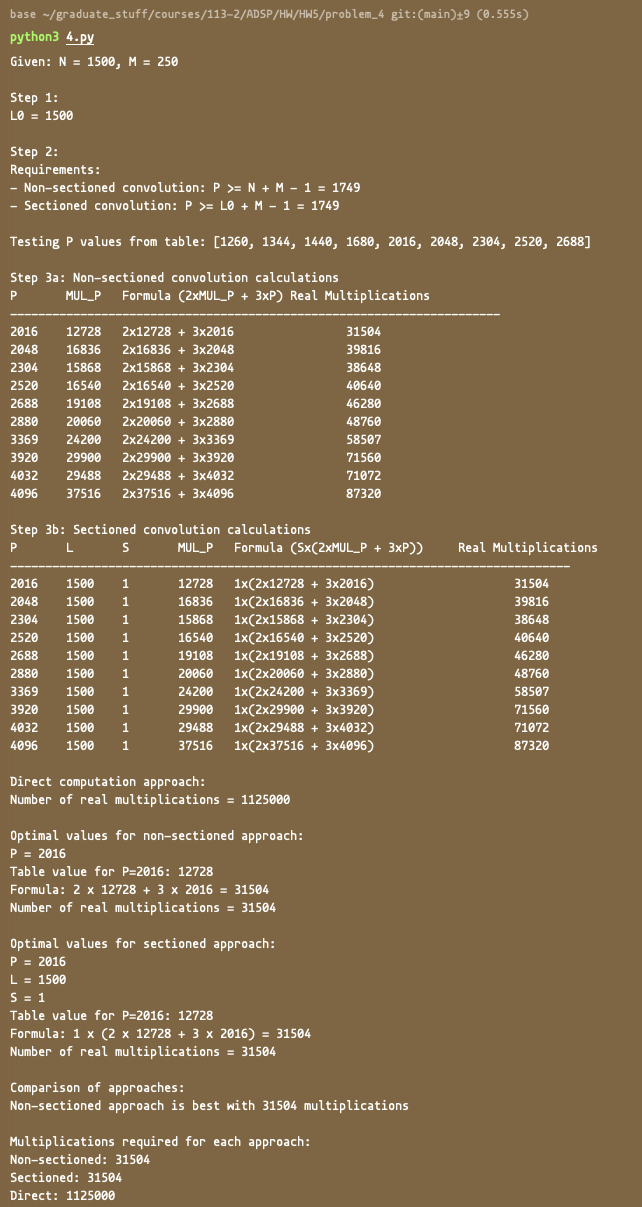
\includegraphics[width=0.9\textwidth]{problem_4/4_a.png}
\end{figure}

From the image, we can see that the optimal condition is: 
\begin{itemize}
    \item (i) Non-sectioned approach
    \item (ii) $P = 2016$
    \item (iii) $31504$ real multiplications
\end{itemize}

\subsection*{(b)}

If $\mathrm{length}(y[n]) = 50$, then we have $N = 1500, \ M = 50$.
The derivation process is shown as the following image:

\begin{figure}[H]
    \centering
    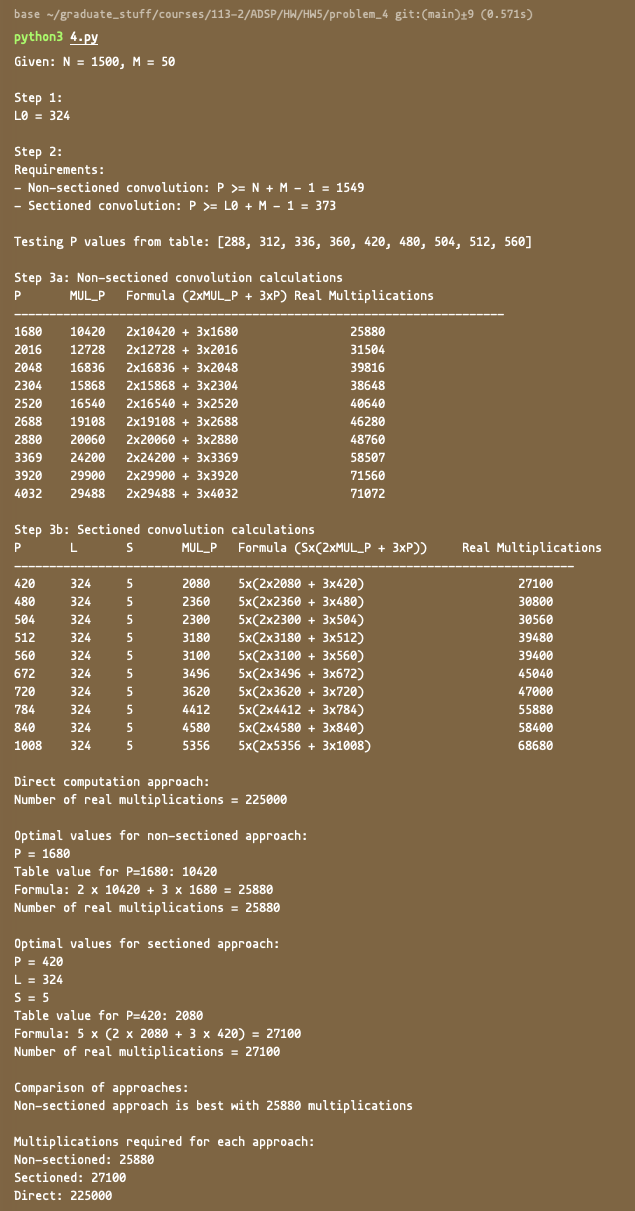
\includegraphics[width=0.9\textwidth]{problem_4/4_b.png}
\end{figure}

From the image, we can see that the optimal condition is: 
\begin{itemize}
    \item (i) Non-sectioned approach
    \item (ii) $P = 1680$
    \item (iii) $25880$ real multiplications
\end{itemize}

% \underline{Direct computing}:

% \begin{align*}
%     3 \times 1500 \times 250 = 1125000
% \end{align*}

% \underline{Non-sectioned convolution}:
% \bigskip

% We have $P \geq 1500 + 250 - 1 = 1749$, before applying the formula, 
% we first calculate $\mathrm{MUL}_{P}$ by the code, 
% and we could get the resulting optimal $P$ as $2016$.
% % Since $1749 = 3 \times 583 = 3 \times 11 \times 53$

% \begin{figure}[H]
%     \centering
%     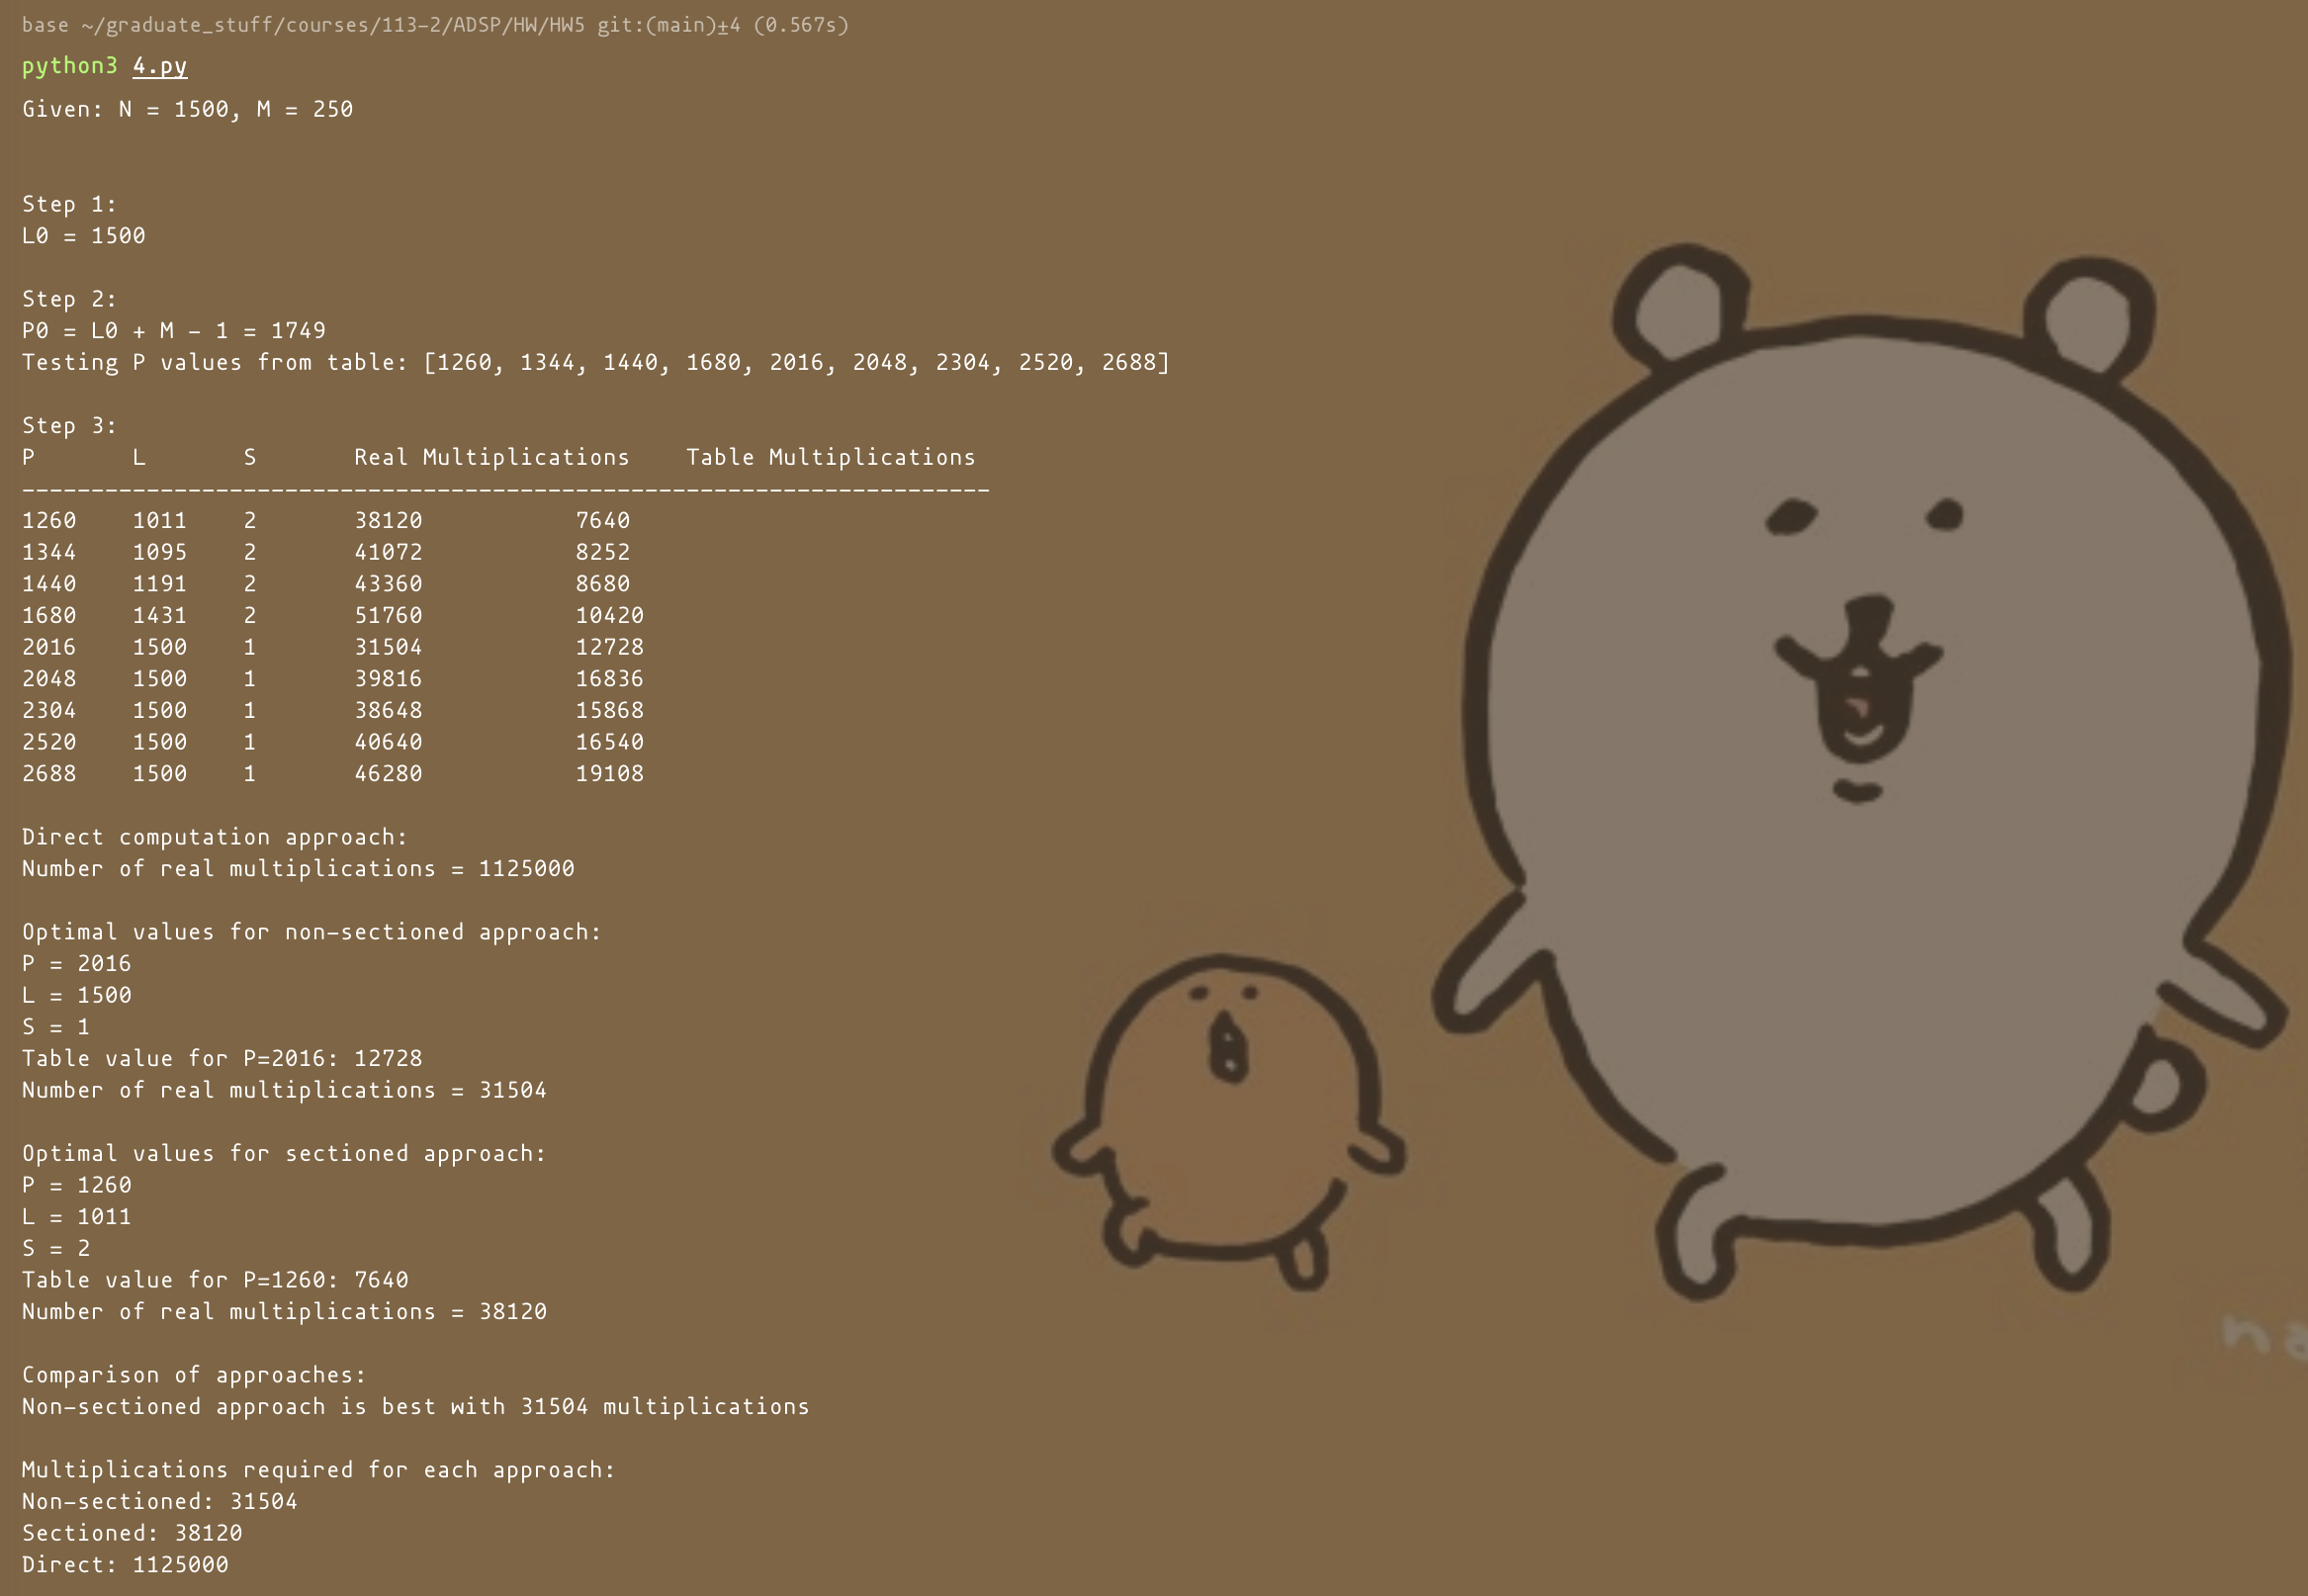
\includegraphics[width=0.9\textwidth]{HW5_img/4_a}
% \end{figure}

% Thus, the number of multiplications using IFFT and FFT with $P = 2016$ ($\mathrm{MUL}_{2016} = 12728$) is:

% \begin{align*}
%     2 \times \mathrm{MUL}_{2016} + 3 \times 2016 = 2 \times 12728 + 3 \times 2016 = 25456 + 6048 = 31504
% \end{align*}

% \underline{Sectioned convolution}:

% \begin{align*}
%     \left\lceil \frac{1500}{250} \right\rceil \times (2 \times \mathrm{MUL}_{2016} + 3 \times 2016) = 6 \times 31504 = 189024
% \end{align*}


\subsection*{(c)}

If $\mathrm{length}(y[n]) = 10$, then we have $N = 1500, \ M = 10$.
The derivation process is shown as the following image:

\begin{figure}[H]
    \centering
    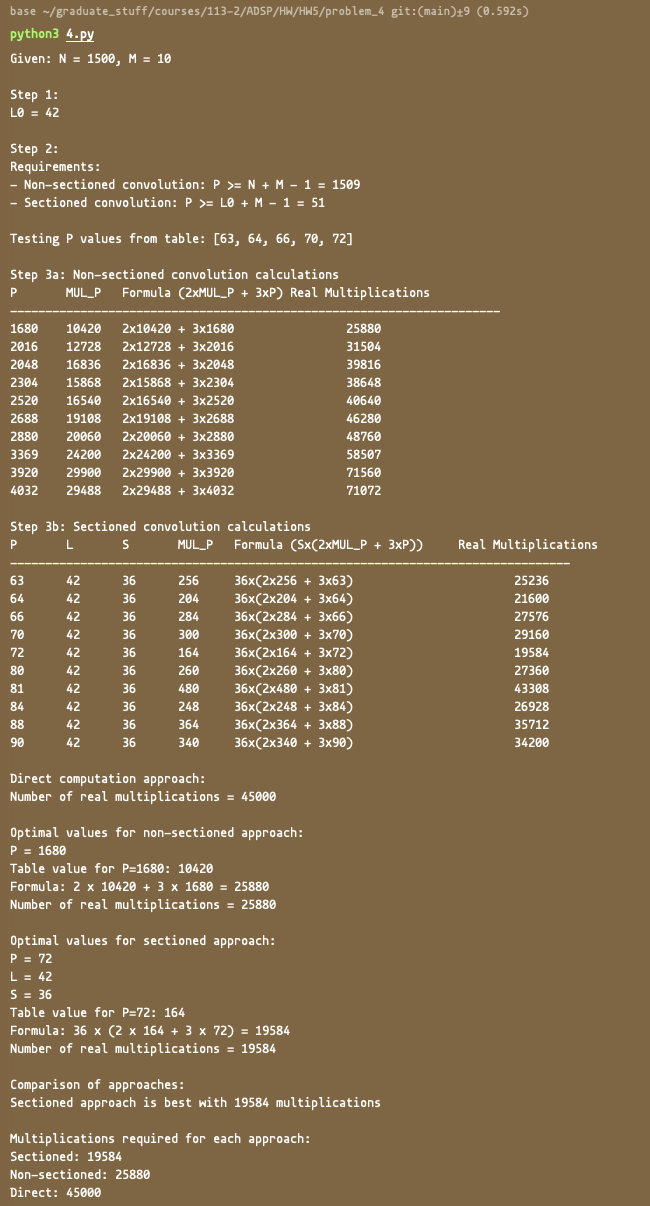
\includegraphics[width=0.9\textwidth]{problem_4/4_c.png}
\end{figure}

From the image, we can see that the optimal condition is: 
\begin{itemize}
    \item (i) Sectioned approach
    \item (ii) $P = 72$
    \item (iii) $19584$ real multiplications
\end{itemize}

\subsection*{(d)}

If $\mathrm{length}(y[n]) = 2$, then we have $N = 1500, \ M = 2$.
The derivation process is shown as the following image:

\begin{figure}[H]
    \centering
    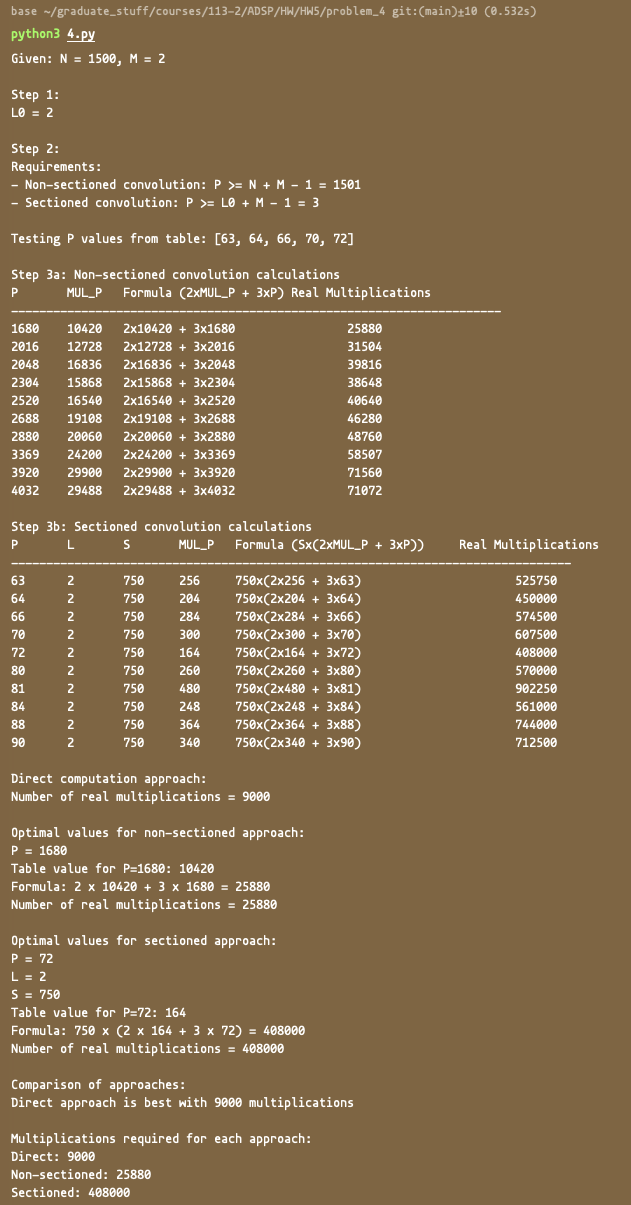
\includegraphics[width=0.9\textwidth]{problem_4/4_d.png}
\end{figure}

From the image, we can see that the optimal condition is: 
\begin{itemize}
    \item (i) Direct approach
    \item (ii) No use of $P$
    \item (iii) $9000$ real multiplications
\end{itemize}

\section*{(5)}

\subsection*{(a)}

% Walsh transform is constituted by $1$s and $-1$s, 
% and would generate lots of the high frequency components, 
% so we could not use completely different $m$s to represent signals of different frequencies.
% Thus, it would not be suitable for Walsh transform to be used for natural signals.

From the lecture note "ADSP\_Write7.pdf", p.483, 
we know that Walsh transform will only become multiplication under logical convolution, 
which is shown as follows:
\bigskip
\begin{tcolorbox}[greenbox, title = Walsh transform: Convolution property]
Let $\Rightarrow$ denote the Walsh transform, and $\star$ denote the logical convolution, 
then we have:

\begin{align*}
    \text{If } f[n] \Rightarrow F[m], \ g[n] \Rightarrow G[m], \ \text{then } f[n] \star g[n] \Rightarrow F[m] \times G[m]
\end{align*}

\end{tcolorbox}

While we do not have this property under linear convolution,
thus, Walsh transform is \underline{not suitable} for calculating the linear convolution.

\subsection*{(b)}

Stair-like signal anaylsis is \underline{suitable} for the Walsh transform, 
since the Walsh transform is a set of orthogonal functions, 
and the stair-like signal is a combination of step functions.

\section*{(6)}

\subsection*{(a)}

For the $32$ point Walsh transform, 
by using the similar method as in the lecture note "ADSP\_Write7.pdf", p.485, 
which is shown below:

\begin{figure}[H]
    \centering
    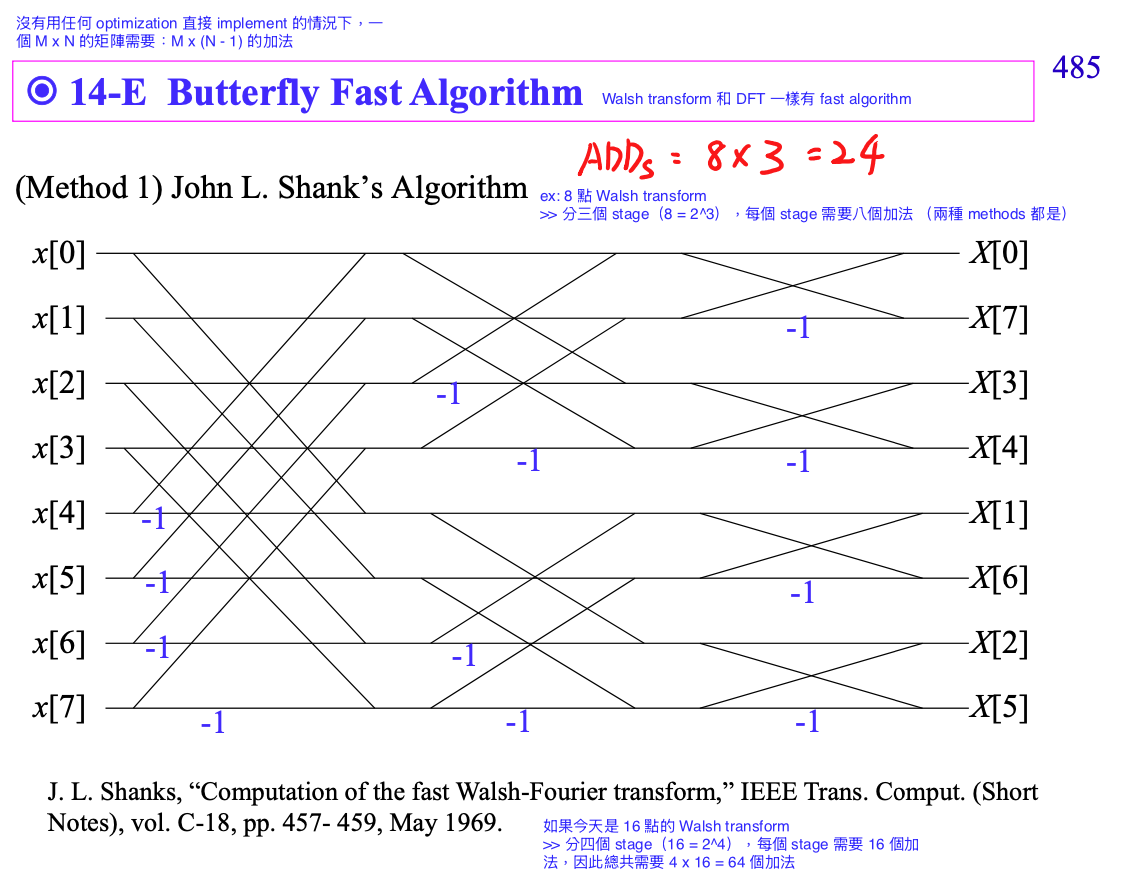
\includegraphics[width=\textwidth]{HW5_img/6_a.png}
\end{figure}

We first need to determine the number of stages needed, 
then determine the number of additions required for each stage.

Since we have $32$ points, which is $2^5$, we need $5$ stages, 
and for each stage, we need $32$ additions, so the total number of additions needed is:

\begin{align*}
    5 \times 32 = 160 \qquad \square
\end{align*}

\subsection*{(b)}

For the $16$ point Haar transform, 
we formulate the matrix as shown in the following lecture note "ADSP\_Write7.pdf", p.490:

\begin{figure}[H]
    \centering
    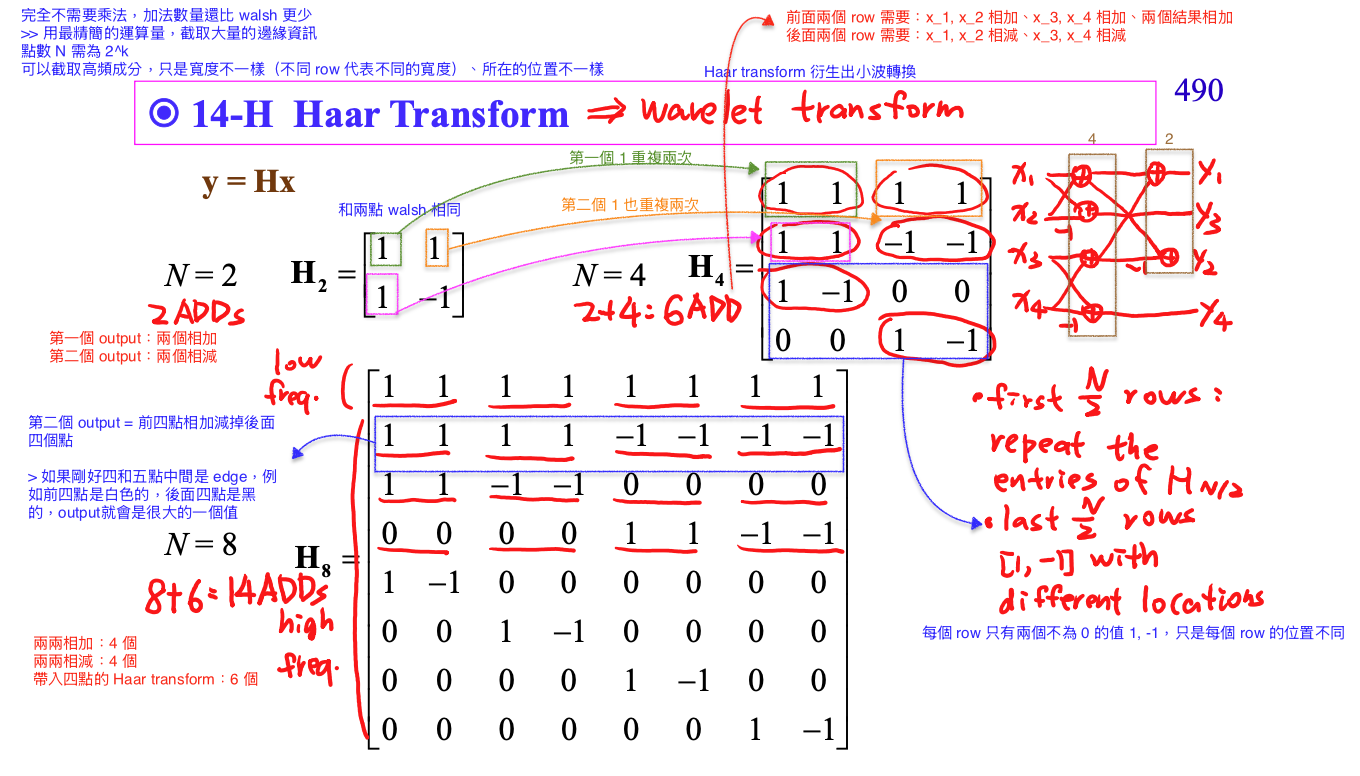
\includegraphics[width=\textwidth]{HW5_img/6_b.png}
\end{figure}

We need the $8$-point Haar transform to realize the $16$-point Haar transform, 
and before applying the $8$-point Haar transform, 
we need every two points to be added and subtracted together, 
which requires:

\begin{enumerate}
    \item $16 \div 2 = 8$ (for additions $x_i + x_{i+1}, \ i = 0, 2, 4, 6, 8, 10, 12, 14$)
    \item $16 \div 2 = 8$ (for subtractions $x_i - x_{i+1}, \ i = 1, 3, 5, 7, 9, 11, 13, 15$)
\end{enumerate}

Thus, the total number of additions needed is:

\begin{align*}
    \underbrace{8}_{x_i + x_{i+1}} + \underbrace{8}_{x_i - x_{i+1}} + \underbrace{8}_{\text{8 point Haar}} = 24 \qquad \square
\end{align*}

\section*{7}

For the subproblems (a) and (b), I use the code as the attached images to generate the results.
Simple explanations are shown in the markdown cells.

\subsection*{(a)}


\begin{figure}[H]
    \centering
    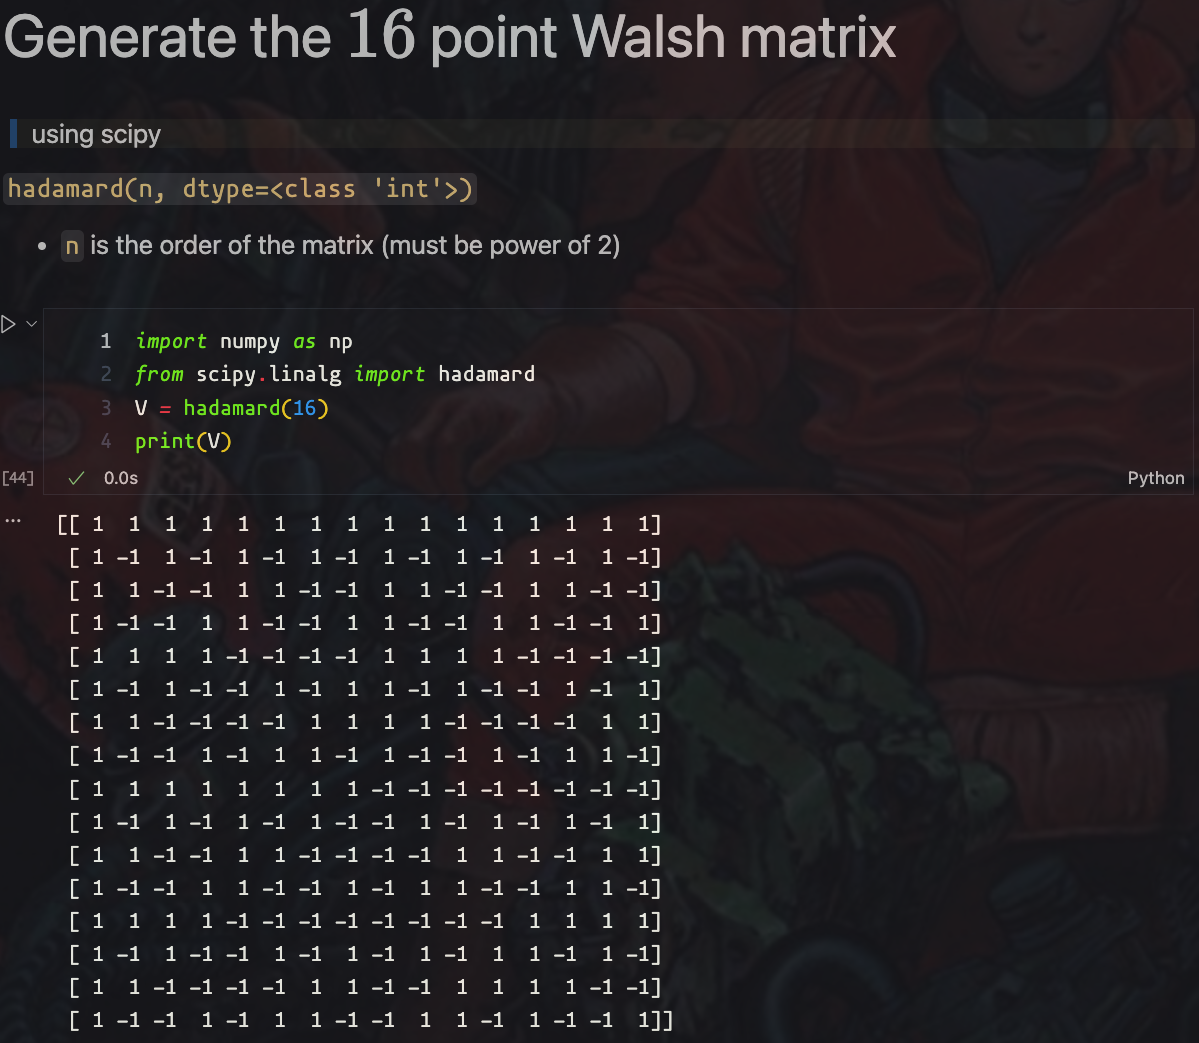
\includegraphics[width=0.8\textwidth]{HW5_img/7/gen_walsh.png}
\end{figure}

\begin{figure}[H]
    \centering
    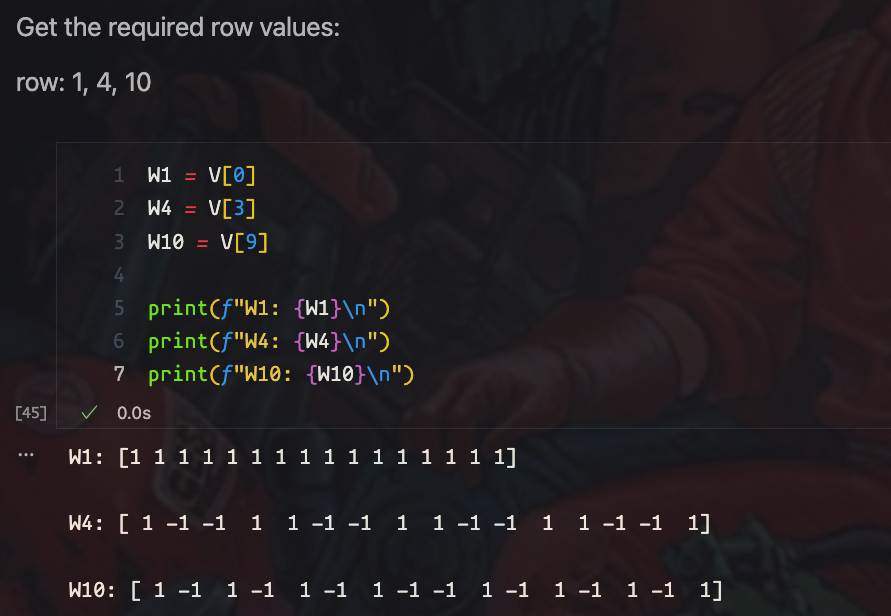
\includegraphics[width=0.8\textwidth]{HW5_img/7/get_required_row.png}
\end{figure}

\begin{figure}[H]
    \centering
    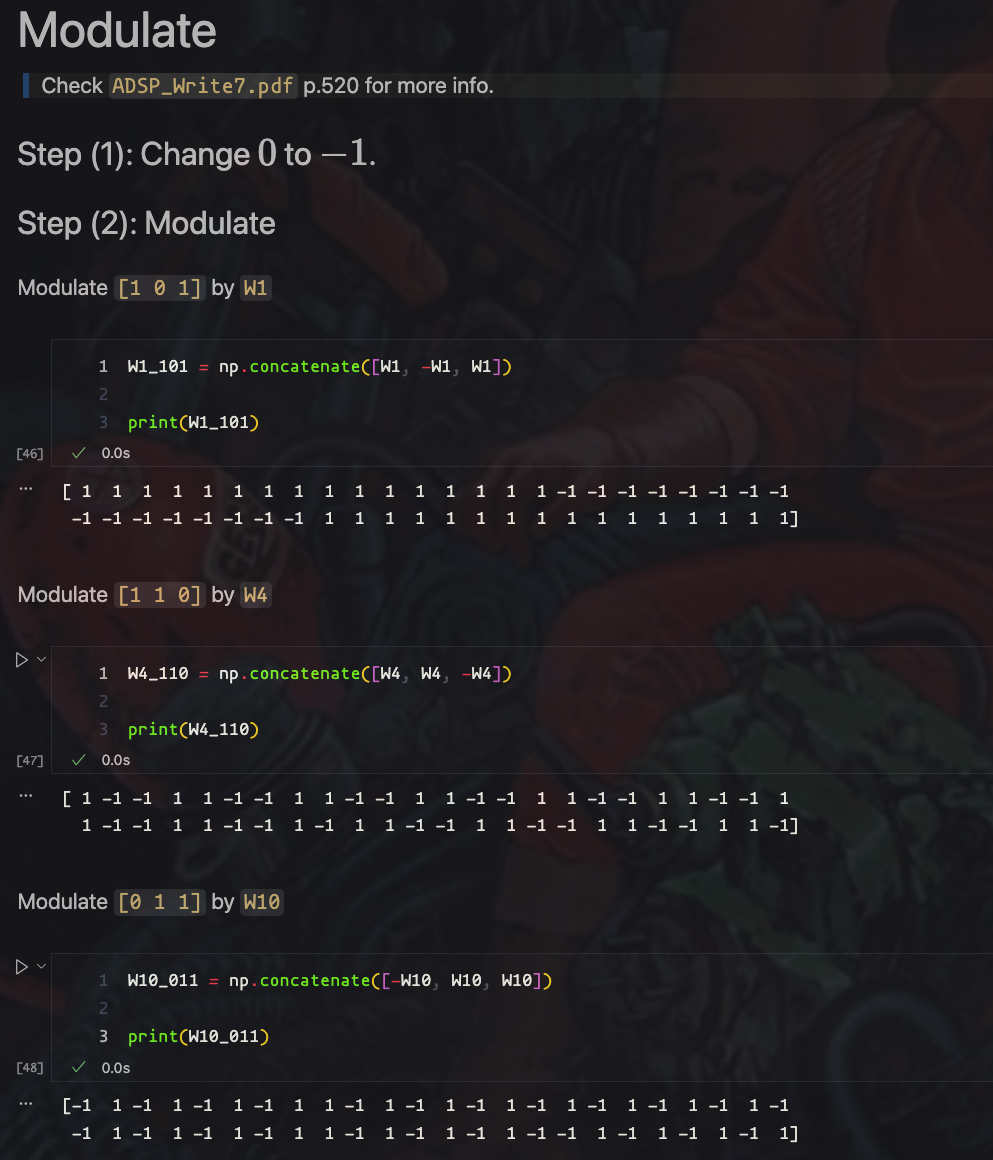
\includegraphics[width=0.8\textwidth]{HW5_img/7/modulate.png}
\end{figure}

And the answer of (a) is as the result of the image below:

\begin{figure}[H]
    \centering
    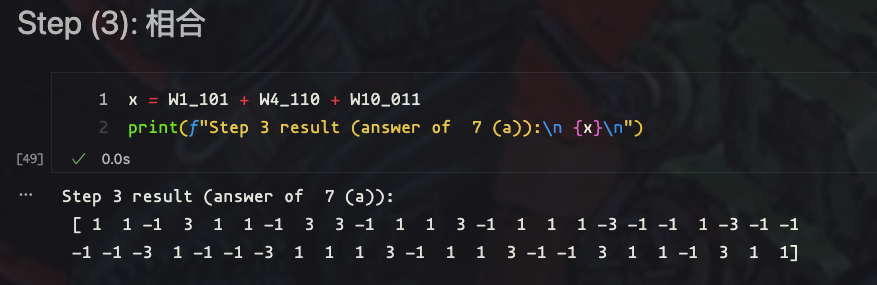
\includegraphics[width=0.8\textwidth]{HW5_img/7/result_a.png}
\end{figure}

Since the image might not be that clear, 
the answer is:

% note: need to add the line \setcounter{MaxMatrixCols}{16} 
\begin{equation*}
    \begin{bmatrix}
    1 & 1 & -1 & 3 & 1 & 1 & -1 & 3 & 3 & -1 & 1 & 1 & 3 & -1 & 1 & 1 \\
    1 & -3 & -1 & -1 & 1 & -3 & -1 & -1 & -1 & -1 & -3 & 1 & -1 & -1 & -3 & 1 \\
    1 & 1 & 3 & -1 & 1 & 1 & 3 & -1 & -1 & 3 & 1 & 1 & -1 & 3 & 1 & 1
    \end{bmatrix} \qquad \square
\end{equation*}


\subsection*{(b)}

\begin{figure}[H]
    \centering
    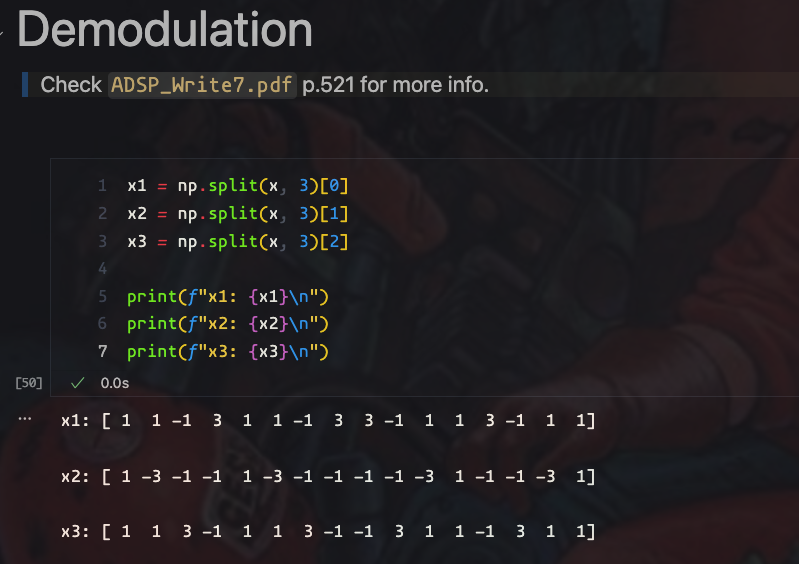
\includegraphics[width=0.8\textwidth]{HW5_img/7/demodulation.png}
\end{figure}

After getting the values of \codeword{x1}, \codeword{x2}, \codeword{x3}, 
we try to recover the original data by the following process, 
note that only the recovery process of \codeword{[1 0 1]} is shown since the rest are the same:

\begin{figure}[H]
    \centering
    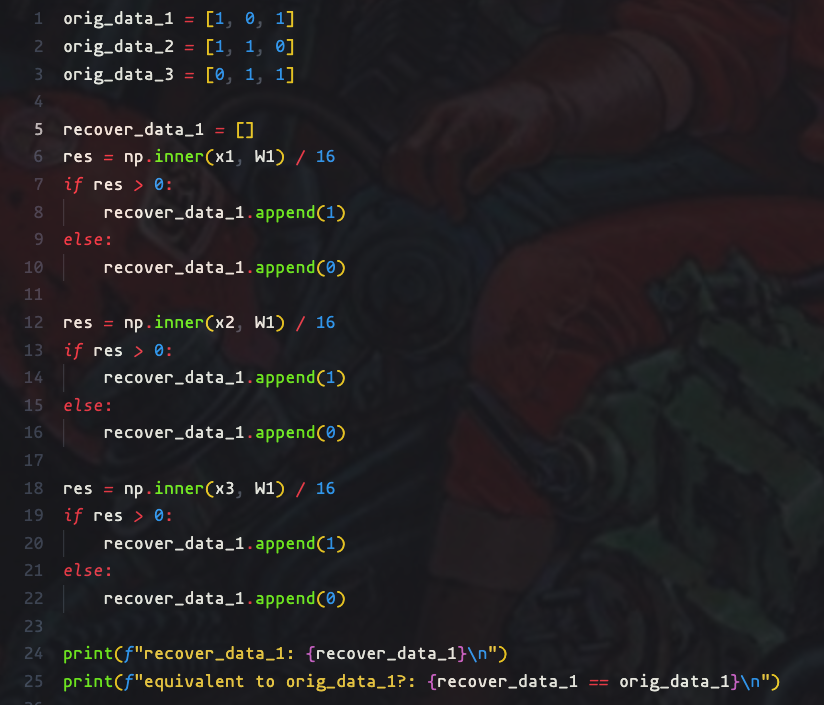
\includegraphics[width=0.8\textwidth]{HW5_img/7/recover_process.png}
\end{figure}

The recover result is as follows:

\begin{figure}[H]
    \centering
    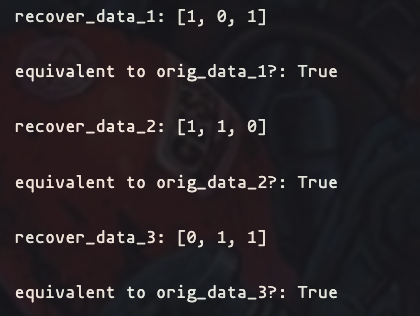
\includegraphics[width=0.5\textwidth]{HW5_img/7/recover_result.png}
\end{figure}

Thus, we can recover the original data by the process shown in the image above.

\subsection*{(c)}

In lecture slide "ADSP\_Write7.pdf", p.522, 
it is said that we can replace Walsh transform with other orthogonal transforms in CDMA, 
hence, it is \underline{suitable} using Haar transform.


\section*{Extra problem (ID ends with $1, 6$)}

How many real multiplications are needed 
when the length of the input function is $100$ points ($N = \mathrm{length}(x[n]) = 100$), 
the filter is $19$ points ($M = \mathrm{length}(h[n]) = 19$), 
and we want to implement it by a $120$ points Fourier transform ($P = 120$)?

\begin{align*}
    &2 \mathrm{MUL}_{120} + 120 \times 3 \\
    = \ & 2 \times 380 + 120 \times 3 \\
    = \ & 760 + 360 \\
    = \ & 1120
\end{align*}

Note that we multiplied $120$ by $3$ since one complex multiplication requires $3$ real multiplications, 
and we got the value of $\mathrm{MUL}_{120} = 380$ by the table in lecture note "ADSP\_Write5.pdf", p.378.


\end{document}